\chapter{Exact Diagonalization}

 	\section{Generalities}
 		
 		Exact diagonalization of the Hamiltonian enables to reach the complete knowledge of a quantum spin system. In general, every finite system can be diagonalized numerically, but limited to small system because computationally inefficient since the size of the basis increases exponentially in the system size. To reach the thermodynamic limit, one needs to seek for block-diagonalization first, as shown on \autoref{fig:blockDiag}. The symmetries are of great interest, and one shall not use group theory to reduce the Hamiltonian but rather introduce a more practical approach. 

 		\begin{figure}[h!]
            \centering
            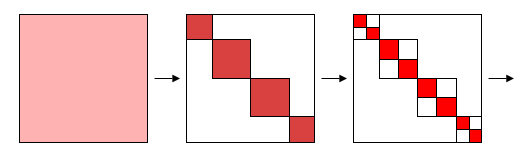
\includegraphics[scale=0.6]{graphs/blockDiag.png}
            \caption{Schematic picture of the block-diadonalization process, reducing their size after applying a symmetry of the Hamiltonian.}
            \label{fig:blockDiag}
        \end{figure}

        For the rest of the discussion, one takes the $S=1/2$ antiferromagnetic Heisenberg Hamiltonian
        \be \begin{split} \mc H &= J \sum_{i=0}^{N-1} \vb* S_i \cdot \vb* S_{i+1} \\ &= J \sum_{i=0}^{N-1} S^z_i S^z_{i+1} + \frac{J}{2} \sum_{i=0}^{N-1} [S^+_i S^-_{i+1} + S^-_i S^+_{i+1}] \end{split} \label{eq:hamED} \ee
        with periodic boundary conditions $\vb* S_N = S_0$. Also, work with the states $\ket{S^z_0,\dotsc, S^z_{N-1}}$.

        Now discuss the symmetries.

    \section{Translation}

    	Define the translation operator as
    	\be T \ket{S^z_0,\dotsc, S^z_{N-1}} = \ket{S^z_{N-1},S^Z_0,\dotsc, S^z_{N-2}} \ee
    	which corresponds tot decreasing the spin index by one at each site. It is important to note that the Hamiltonian \eqref{eq:hamED} is invariant under the action of $T$, that is
    	\be [\mc H, T] = 0 \label{eq:commuteEDHT} \ee
    	Therefore, one can construct the momentum states $\ket{a(k)}$ as
    	\be T \ket{a(k)} = e^{ik} \ket{a(k)} \ee
    	with the momentum allowed being
    	\be k = \frac{2\pi}{N}m \qq{with} m = -N/2 +1,\dotsc, N/2 \ee
    	since $T^N=\mathbb 1$ and lattice constant equal to $1$. Then, it is possible to introduce a reference state $\ket a$, which is a single state in the $z$-component basis, giving
    	\be \ket{a(k)} = \frac{1}{\sqrt{N_a}} \sum_{r=0}^{N-1} e^{-ikr}T^r\ket a \ee
    	To find a complete set of normalizable orthogonal states, start by seeing that 
    	\be \braket{a(k)}{b(k)} = 0 \iff T^r \ket a \neq \ket b \ \forall r \ee
    	Hence, only one of the states in the set of translated states $T^r \ket a$ can be chosen as a representative.

    	If all $T^r \ket a$ are distinct, then $N=N_a$. But if the periodicity is less than $N$, it can be chosen as the smallest $R_a$ such that
    	\be T^{R_a} \ket a = \ket a \qq{with} R_a \in \{1,\dotsc,N\} \ee
    	To correctly relate the normalization factor to $R_a$ instead of restricting the summation up to $r=R_a$, take the sum of the phases
    	\be \begin{split} F(k,R_a) &= \sum_{n=0}^{N/R_a -1} e^{-iknR_a} \\ &= \begin{cases} N/R_a & \text{if } kR_a \equiv 0 \mod 2\pi \\ 0 & \text{otherwise} \end{cases} \end{split} \ee
    	Thus
    	\be N_a = R_a \abs{F(k,R_a)}^2 \ee
    	This means that $F(k,R_a)=0$ is not allowed, and hence for a given $\ket a$, $k = \frac{2\pi}{R_a}m$ with $m=0, \dotsc, R_a-1$ and
    	\be N_a =\frac{N^2}{R_a} \ee

    	Now construct the Hamiltonian matrix in the momentum basis. To simplify, define
    	\be \mc H = J \sum_{j=0}^N \mc H_j \ee
    	with
    	\be \mc H_0 = \sum_{i=0}^{N-1} S^z_i S^z_{i+1} \qq{and} \mc H_j = \frac{1}{2} [S^+_j S^-_{j+1} + S^-_j S^+_{j+1}] \ee
    	and set $J=1$. Then, according to \eqref{eq:commuteEDHT}, write
    	\be \begin{split} \mc H \ket{a(k)} &= \frac{1}{\sqrt{N_a}} \sum_{r=0}^{N-1} e^{-ikr}T^r \mc H \ket a \\ &= \frac{1}{\sqrt{N_a}} \sum_{j=0}^N \sum_{r=0}^{N-1} e^{-ikr}T^r \mc H_j \ket a \end{split} \ee
    	This allows to write
    	\be \begin{split} \mc H_j \ket a &= h_j(a) \ket{b'_j} \\ &= h_j(a) T^{-l_j} \ket{b'_j} \qq{with} l_j = 0,\dotsc, N-1 \end{split} \ee
    	giving finally
    	\be \begin{split} \mc H \ket{a(k)} &= \sum_{j=0}^N \frac{h_j(a)}{\sqrt{N_a}} \sum_{r=0}^{N-1} e^{-ikr}T^{r-l_j} \ket{b_j} \\ &= \sum_{j=0}^N h_j(a) e^{-ikl_j}\sqrt{\frac{N_{b_j}}{N_a}} \ket{b_j(k)} \end{split} \ee
    	Therefore, the matrix elements are
    	\be \mel{b_j(k)}{\mc H_j}{a(k)} = h_j(a) e^{-ikl_j} \sqrt{\frac{N_{b_j}}{N_a}} \ee
    	Overall, trading $h_j(a)$ by the values of the diagonal and off-diagonal elements, get
    	\be \begin{split} \mel{a(k)}{\mc H_0}{a(k)} &= \sum_{j=1}^N S^z_j S^z_j \\ \qq{and} \mel{b_j(k)}{\mc H_{j>0}}{a(k)} &= \frac{e^{-ikl_j}}{2} \sqrt{\frac{R_a}{R_{b_j}}} \end{split} \ee

    \section{Inversion}

    	Define the magnetization in the direction of the quantization axis $z$ as
    	\be m_z = \sum_{j=0}^{N-1} S_j^z \ee
    	For the case $m_z=0$ for $N$ even, one can block-diadonalize using a discrete subspace of all the possible spin-rotations, the spin inversion symmetry that is the invariance with respect to flipping all the spins. It is defined as
   		\be Z \ket{S^z_0,\dotsc, S^z_{N-1}} = \ket{-S^Z_0,\dotsc, -S^z_{N-1}} \ee
   		For this operator, one has $Z^2=\mathbb 1$. It is thus possible to block-diadonalize the Hamiltonian in the $m_z=0$ sector. Denote by$z=\pm 1$ the eigenvalues of $Z$. Since
   		\be [Z,T] = 0 \ee
   		one can further reduce the size of the blocks by writing first
   		\be \ket{a(k,z)} = \frac{1}{\sqrt{N_a}} \sum_{r=0}^{N-1} e^{-ikr}T^r[1+zZ]\ket a \ee
   		with the normalization constant
   		\be N_a = \frac{2N^2}{R_a} \begin{cases} 1 & T^m Z \ket a \neq \ket a \ \forall m \\ 1 + z \cos km & T^m Z \ket a = \ket a \end{cases} \ee 
   		The Hamiltonian then acts as
   		\be \mc H_j \ket a = h_j(a) Z^{g_j} T^{-l_j} \ket{b_j} \qq{with} g_j = 0,1 \ee
   		giving the matrix elements
   		\be \mel{b_j(k,z)}{\mc H_j}{a(k,z)} = h_j(a)z^{g_j} e^{-ikl_j} \sqrt{\frac{N_{b_j}}{N_a}} \ee
   		valid $\forall k$

   	\section{Parity}

   		The Hamiltonian also commutes with the parity operator
   		\be P \ket{S^z_0,\dotsc, S^z_{N-1}} = \ket{S^Z_{N-1},\dotsc, -S^z_1, S^z_0} \ee
   		with $P^2=\mathbb 1$ and thus the eigenvalues $p=\pm 1$. But
 		\be [P,T] \neq 0 \ee
 		in general, but they commute for $k=0,\pi$. To show that, write
 		\be \ket{a(k,p)} = \frac{1}{\sqrt{N_a}} \sum_{r=0}^{N-1} e^{-ikr}T^r[1+pP]\ket a  \label{eq:akpEDP} \ee
 		Since $PT = T^{-1}P$, one has
 		\be \begin{split} P\ket{a(k,p)} &= \frac{1}{\sqrt{N_a}} \sum_{r=0}^{N-1} e^{-ikr}T^-r[1+P]\ket a \\ &= p\frac{1}{\sqrt{N_a}} \sum_{r=0}^{N-1} e^{ikr}T^r[1+pP]\ket a \end{split} \ee
 		which is \eqref{eq:akpEDP} for $k=0,\pi$ and in this cases the block-diadonalization can be made using the both parity and translational invariance.

 		But one is interesting in block-diadonalization for the general case. Hence, it is possible to mix momentum states with $\pm k$ and thereby consider the semi-momentum states
 		\be\ket{a^\sigma(k)} = \frac{1}{\sqrt{N_a}} \sum_{r=0}^{N-1} C^\sigma_k(r) T^r\ket a \ee
 		where $\sigma$ stands for the spin $\sigma = \pm 1$ and
 		\be C_k^\sigma (r) = \begin{cases} \cos kr & \sigma = +1 \\ \sin kr & \sigma = -1 \end{cases} \ee
 		Consider only half of the first Brillouin zone $0 \leq k \leq \pi$. With some workaround not interesting here for the normalization and orthogonality, one can find
 		\be \ket{a^\sigma(k,p)} = \frac{1}{\sqrt{N^\sigma_a}} \sum_{r=0}^{N-1} C^\sigma_k (r) [1+pP] T^r\ket a \ee
 		and pursue the computation to fanilly find the matrix elements for the semi-momentum states.

 	\section{The Lanczos method}

 		Performing complete diagonalization becomes rapidly time consuming. It is therefore sometimes useful to restrict to only find the ground state and possibly some excited states. The Lanczos algorithm is a Krylov-space technique that allows this. \\

 		The Krylov space is a subspace of the full Hilbert space such that the low-lying excited states are well approximated within it. Consider a random state $\ket \psi$ and $M$ the dimension of the full Hilbert space. Then express it as a linear combination of the eigenstates $\ket{\psi_n}$ of the Hamiltonian
 		\be \begin{split} \mc H^\Lambda \ket \psi &= \sum_{n=0}^{M-1} c_n E^\Lambda_n \ket{\psi_n} \\ &= c_\text{max} E^\Lambda_\text{max}\left[ \ket{\psi_\text{max}} + \sum_{n \neq n_\text{max}} \frac{c_n}{c_\text{max}} \left(\frac{E_n}{E_\text{max}} \right)^2 \ket{\psi_n} \right] \end{split} \ee
 		For a large $\Lambda$, the state with eigenvalue $\abs{E_\text{max}}$ will dominate the sum provided $c_\text{max}\neq 0$ obviously. Hence, acting with the Hamiltonian many times will project out the eigenvector with the largest-magnitude eigenvalue. To reach the ground state $\ket{\psi_0}$, one must apply $(\mc -c)^\Lambda$ instead, with $c$ ensuring that $\abs{E_0-c}>\abs{E_{M-1}-c}$, typically $c=E_\text{max}$. In what follows, assume such constant is already absorbed in the Hamiltonian if needed.

 		A more efficient way to obtain the ground state for $\Lambda \to \infty$ is to consider the whole subspace spanned by the set of $\mc H^m \ket \psi$ with $m=0, \dotsc, \Lambda$. This composes the Krylov space. The Lanczos method consists in constructing an orthogonal basis using linear combination of the states in the Krylov space such that the Hamiltonian is tridiagonal in it. This procedure is like the Gram-Schmidt orthonormalization. Start with a random state normalized $\ket{\phi_0}$. Then
 		\be \ket{\phi_1} = \frac{1}{\sqrt{N_1}}\underbrace{[\mc H \ket{\phi_0} - a_0\ket{\phi_0}]}_{\ket{\gamma_1}} \ee
 		so that $\braket{\phi_0}{\phi_1} = 0$ and $\ev{\mc H}{\phi_0} = a_0$, which gives $N_1 = \braket{\gamma_1}{\gamma_1}$. Repeat the procedure to have in general
 		\be \ket{\phi_{m+1}} = \frac{1}{\sqrt{N_{m+1}}} \underbrace{[\mc H \ket{\phi_m} - a_m \ket{\phi_m} - \sqrt{N_m}\ket{\phi_{m-1}}]}_{\ket{\gamma_{m+1}}} \ee
 		with
 		\be a_m = \ev{\mc H}{\phi_m} \qq{and} N_m = \braket{\gamma_m}{\gamma_m} \ee
 		requiring it to be orthogonal to all the previous states. Indeed
 		\be \begin{split} \braket{\phi_{m+1}}{\phi_{m-k}} &= \frac{1}{\sqrt{N_{m+1}}} \mel{\phi_m}{\mc H}{\phi_{m-k}} \\ &= \frac{1}{\sqrt{N_{m+1}}} [\sqrt{N_{m-k+1}}\braket{\phi_m}{\phi_{m-k+1}} \\ &+ a_{m-k} \braket{\phi_m}{\phi_{m-k}} \\ &+ \sqrt{N_{m-k}}\braket{\phi_m}{\phi_{m-k-1}}] \\ &=0 \end{split} \ee
 		supposing all the previously generated states are orthogonal to each other. Therefore
 		\be \mc H \ket{\phi_m} = \sqrt{N_{m+1}} \ket{\phi_{m+1}} + a_m \ket{\phi_m} + \sqrt{N_m}\ket{\phi_{m-1}} \ee
 		or writing in tridiagonal form, with $b_m = \sqrt{N_{m+1}}$
 		\be \mc H \doteq \pmqty{a_0 & b_0 & & & \\ b_0 & a_1 & b_1 & & \\ & b_1 & a_2 & \ddots & \\ & & \ddots & \ddots &} \ee





